\pagebreak
\section{Logarithmus}\label{sec:E-Funktion/Logarithmus}
Betrachtet man folgendes, könnte auffallen, dass es einen Beziehung zwischen $n$,$b$ und $r$ geben könnte.  
\begin{align*}
	b^n=r
\end{align*}
\paragraph{Die Potenz} beschreibt zunächst den Weg, wie man zu $r$ kommt. Dies erfolgt durch das Potenzieren der Basis $b$ mit dem Exponenten $n$
\paragraph{Die Wurzel} beschreibt die Beziehung zwischen $r$ und $n$ und ergibt abschließend $b$
\paragraph{Der Logarithmus} beschreibt die Beziehung zwischen der Basis $b$ und dem Ergebnis $r$.
\begin{figure}[h]
	\centering
	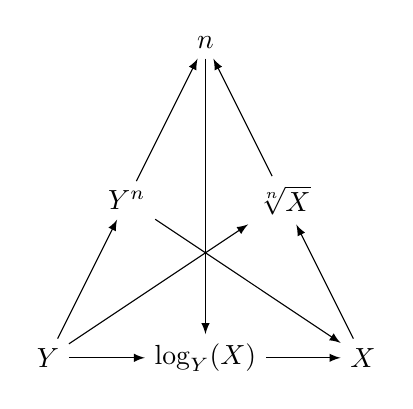
\begin{tikzpicture}[>=latex,font=\sffamily]
  % Knoten
  \node (b) at (0,0) {$Y$};
  \node (bn) at (1,2) {$Y^n$};
  \node (E) at (4,0) {$X$};
  \node (n) at (2,4) {$n$};
  \node (nrootE) at (3,2) {$\sqrt[n]{X}$};
  \node (logbE) at (2,0) {$\log_Y(X)$};

  % Pfeile
  \draw[->] (b) -- (bn) node[midway,left] {};
  \draw[->] (bn) -- (n) node[midway,left] {};
  \draw[->] (E) -- (nrootE) node[midway,right] {};
  \draw[->] (nrootE) -- (n) node[midway,right] {};
  \draw[->] (b) -- (logbE) node[midway,below] {};
  \draw[->] (logbE) -- (E) node[midway,below] {};

  % Diagonale Linien
  \draw[->] (b) -- (nrootE);
  \draw[->] (bn) -- (E);
  \draw[->] (n) -- (logbE);
  % Beschriftungen
\end{tikzpicture}
	\caption{Auswirkung von $a$ auf den Graphen}
\end{figure}
\subsubsection{Entstehung}\label{sec:E-Funktion/Logarithmus/Entstehung}
Dem Logarithmus liegt die Mercator-Reihe zugrunde und ist lediglich eine Approximation... 
%TODO Hier fehlt eine Erklärung
\subsubsection{Bedeutung}\label{sec:E-Funktion/Logarithmus/Bedeutung}
Durch die Eigenschaften des Logarithmus kann man sagen, dass dieser das Verhältnis zwischen 
\subsubsection{Anwendung}\label{sec:E-Funktion/Logarithmus/Anwendung}
\subsection{Logarithmus naturalis} Der Logarithmus naturalis ist der Logarithmus zu der Basis $e$ und wird als verkürzte Schreibweise für $log_e(n)$ genutzt. 
\subsection{Logarihtmus Gesetzt}
Logarihtmusgesetze sind eine der Grundlegenden Vorrausetzung, um mit dem Logarithmus rechnen zu können. 
\subsubsection{1. Logrithmusgesetz}
\begin{align*}
	ln(x\cdot y)=ln(x)+ln(y)
\end{align*}
\subsubsection{2. Logrithmusgesetz}
\begin{align*}
	ln\left(\frac{x}{y}\right)=ln(x)-ln(y)
\end{align*}
\subsubsection{2. Logrithmusgesetz}
\begin{align*}
	ln(x^t)=t\cdotln(x)
\end{align*}
\pagebreak
\section{Ableitung des Logarithmus Naturalis}
Genauso wie andere Funktion besitzt der $ln$ eine Ableitung. Die Besonderheit ist hierbei allerdings, dass die Ableitung des $ln(x)$ immer $\frac{1}{x}$ ist. Als Erklärung kann man sich folgendes Anschauen:
\begin{align*}
	x&=e^{ln(x)}\tag{Ableiten auf beiden Seiten}\\
	1&=(ln(x))'\cdot e^{ln(x)}\tag{Beide Seiten vereinfachen}\\
	1&=(ln(x))'\cdot x\tag{Durch $x$ dividieren}\\
	\frac{1}{x}&=(ln(x))'\\	
\end{align*}
\pagebreak
\section{Verschiebung \& Streckung des $ln(x)$}
Genauso wie die $e$-Funktion lässt sich der $ln$ ebenfalls im Koordinatensystem durch verschiedene Parameter modelieren. Hierbei kommt die Normalform des $ln(x)$ zum Einsatz.
\[f(x)=a\cdot ln(b\cdot(x-c))+d\]
\subsubsection{$a$ - Streck- oder Stauchungsfaktor}
Der Streck- oder Stauchungsfaktor sorgt für eine Streckung oder Stauchung an der $Y$-Achse. Der Grund hierfür ist, dass zunächst die Werte auf $Y$-Achse mit dem $ln$ berechnet werden und anschließend mit $a$ multipliziert werden. Somit bleibt ebenfalls die Nullstelle erhalten, da sich beim Multiplizieren mit Null (wenn man in $ln(x)$ die Zahl $1$ einsetzt) immer Null ergibt. 
\begin{figure}[h]
\centering
	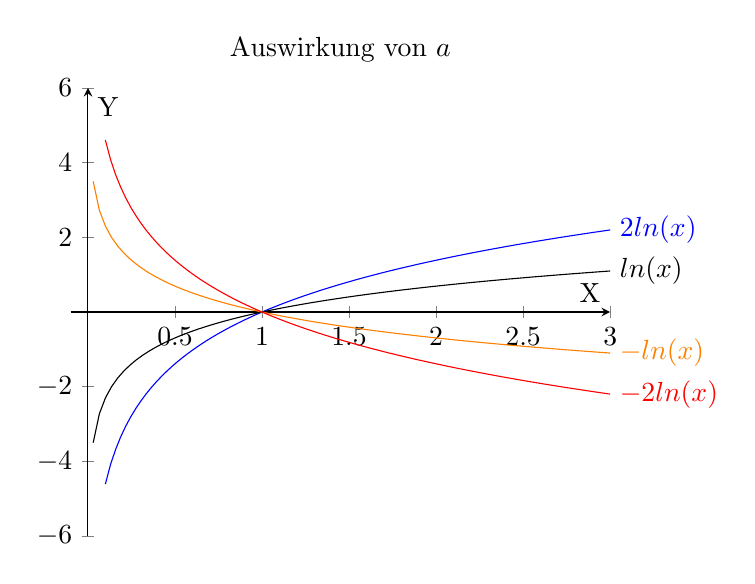
\begin{tikzpicture}
		\begin{axis}[
		title={Auswirkung von $a$},
		axis lines=middle,
		clip=false,
		xlabel={X},
		ylabel={Y},
		xmin=-0.1,
		xmax=3,
		ymin=-6,
		ymax=6
		]
		\addplot[domain=0.1:3,blue, samples=100]{2*ln(x)} node[right,pos=1]{$2ln(x)$};
		\addplot[domain=-0.5:3,black,samples=100]{ln(x)}node[right,pos=1]{$ln(x)$};
		\addplot[domain=-0.5:3,orange,samples=100]{-ln(x)}node[right,pos=1]{$-ln(x)$};
		\addplot[domain=0.1:3,red,samples=100]{-2*ln(x)}node[right,pos=1]{$-2ln(x)$};
		\end{axis}
	\end{tikzpicture}
	\caption{Auswirkung von $a$ auf den Graphen}
\end{figure}
\pagebreak
\subsubsection{$b$ - Streck- oder Stauchfaktor}
Der Koeffizent $b$ ist ebenfalls ein Stauchungs- oder Streckfaktor im Bezug auf den Graphen. Allerdings streckt dieser den Graphen auf der $X$-Achse, indem er die $x$-Werte bevor sie durch den $ln$ nacher die $Y-Wert$ ergeben, multipliziert. Das Bedeutet, dass die $Y$- Werte, die eigentlich an einem anderen Wertepaar erst erreicht werden mit einem davorliegenden $x$ erreicht werden. Außerdem spiegelt man mit diesem Faktor den Graphen an der $Y$-Achse.  
\begin{paracol}{2}
	\begin{flushleft}
	\begin{beispiel}
	\begin{align*}
		f(x)=ln(x)\\
		f(3)=ln(3)\\
		f(3)=1.09\\
	\end{align*}
\end{beispiel}
	\end{flushleft}	
\switchcolumn
	\begin{flushright}
		\begin{beispiel}
	\begin{align*}
		f(x)=ln(2x)\\
		f(3)=ln(2\cdot3)\\
		f(3)=1.79\\
	\end{align*}
\end{beispiel}
	\end{flushright}
\end{paracol}
\begin{figure}[h]
\centering
	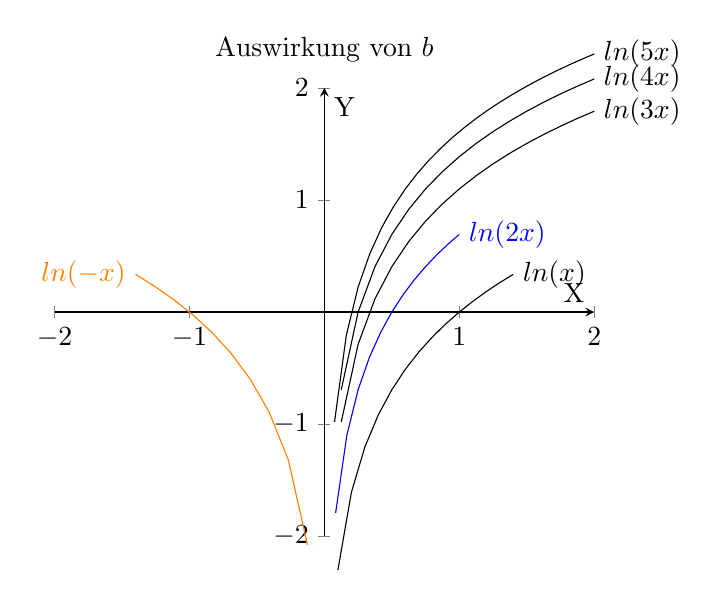
\begin{tikzpicture}
		\begin{axis}[
		title={Auswirkung von $b$},
		axis lines=middle,
		clip=false,
		xlabel={X},
		ylabel={Y},
		xmin=-2,
		xmax=2,
		ymin=-2,
		ymax=2
		]
		\addplot[domain=-1:1,blue]{ln(2*x)} node[right,pos=1]{$ln(2x)$};
		\addplot[domain=-1:1.4,black]{ln(x)}node[right,pos=1]{$ln(x)$};
		\addplot[domain=-1.4:2,orange]{ln(-x)}node[left,pos=0]{$ln(-x)$};
		\addplot[domain=-1:2,black]{ln(3*x)}node[right,pos=1]{$ln(3x)$};
		\addplot[domain=-1:2,black]{ln(4*x)}node[right,pos=1]{$ln(4x)$};
		\addplot[domain=-0.1:2,black]{ln(5*x)}node[right,pos=1]{$ln(5x)$};
		\end{axis}
	\end{tikzpicture}
	\caption{Auswirkung von $b$ auf den Graphen}
\end{figure}
\pagebreak
\subsubsection{$c$-Verschiebung auf $X$-Achse} Mit $c$ lässt sich der Graph auf der $Y$-Achse verschieben. Ist $c<0$ verschiebt sich hierbei der Graph nach rechts. Ist $x>0$ verschiebt er sich nach links.

\begin{figure}[h]
\centering
	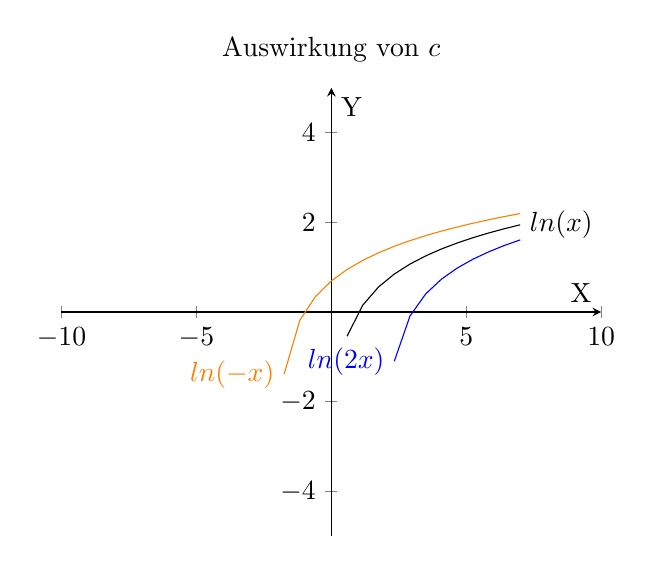
\begin{tikzpicture}
		\begin{axis}[
		title={Auswirkung von $c$},
		axis lines=middle,
		clip=false,
		xlabel={X},
		ylabel={Y},
		xmin=-10,
		xmax=10,
		ymin=-5,
		ymax=5
		]
		\addplot[domain=-7:7,blue]{ln(x-2)} node[left,pos=0]{$ln(2x)$};
		\addplot[domain=-7:7,black]{ln(x)}node[right,pos=1]{$ln(x)$};
		\addplot[domain=-7:7,orange]{ln(x+2)}node[left,pos=0]{$ln(-x)$};
		\end{axis}
	\end{tikzpicture}
	\caption{Auswirkung von $c$ auf den Graphen}
\end{figure}
\pagebreak
\subsubsection{$b$ - Y-Achsenverschiebung}
Der Summand $b$ sorgt für eine $Y$-Achsenverschiebung, da zu den $X$-Werten jeweils ein gewisser Wert addiert oder subtrahiert wird.
\begin{figure}[h]
\centering
	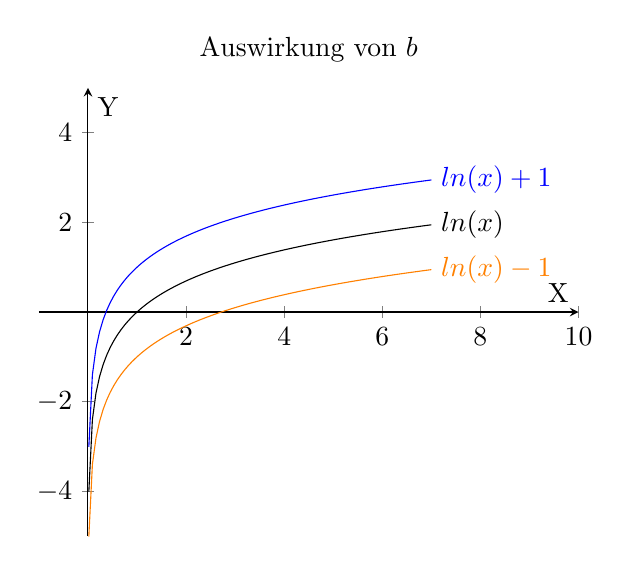
\begin{tikzpicture}
		\begin{axis}[
		title={Auswirkung von $b$},
		axis lines=middle,
		clip=false,
		xlabel={X},
		ylabel={Y},
		xmin=-1,
		xmax=10,
		ymin=-5,
		ymax=5
		]
		\addplot[domain=-0.2:7,blue, samples=100]{ln(x)+1} node[right,pos=1]{$ln(x)+1$};
		\addplot[domain=-0.2:7,black, samples=100]{ln(x)}node[right,pos=1]{$ln(x)$};
		\addplot[domain=-0.2:7,orange, samples=100]{ln(x)-1}node[right,pos=1]{$ln(x)-1$};
		\end{axis}
	\end{tikzpicture}
	\caption{Auswirkung von $b$ auf den Graphen}
\end{figure}
\pagebreak
\section{Inverse von $ln(x)$}
Um die Inverse des $ln(x)$ zu bilden muss die Definitionsmenge und Wertemenge vertauschst werden und anschließend äquvalent umgeformt werden. 

\begin{beispiel}
	\begin{align*}
		f(x)=5\cdot2^x\tag{$f(x)$ zu $y$ umschreiben}\\
		y=5\cdot2^x\tag{Umformen nach $x$}\\
		y=5\cdot 2^x\tag{Dividieren von $5$}\\
		\frac{y}{5}=2^x\tag{Logarithmieren}\\
		ln\left(\frac{y}{5}\right)=ln(2^x)\tag{3. Logarithmusgesetz}\\
		ln\left(\frac{y}{5}\right)=x\cdot ln(2)\tag{Dividieren $ln(2)$}\\
		\frac{ln\left(\frac{y}{5}\right)}{ln(2)}=x\\
		\Rightarrow f^{-1}(x)=\frac{ln\left(\frac{x}{5}\right)}{ln(2)}
		\end{align*}
\end{beispiel}
\section{Begrenztes Wachstum}
Es gibt Sachverhalte, die erfodern, dass eine e-Funktion/Exponential Funktion nicht in ihrer ursprünglichen Form vorliegt. Dass bedeutet, dass nicht jeder Sachverhalt gleich mit einer Funktion, der Form $f(x)ae^{kx}$ oder $f(x)=a\cdot b^x$ modeliert werden kann. So eignet sich das  Beispiel eines Glasses Milch, der in einen Raum gestellt wird und somit sich Temperatur der auf die Raumtemperatur angleicht. Den Verlauf der Temperatur darzustellen in Abhängikeit der Zeit ergibt nur auf eine Art Sinn.
\begin{figure}[h]
\centering
	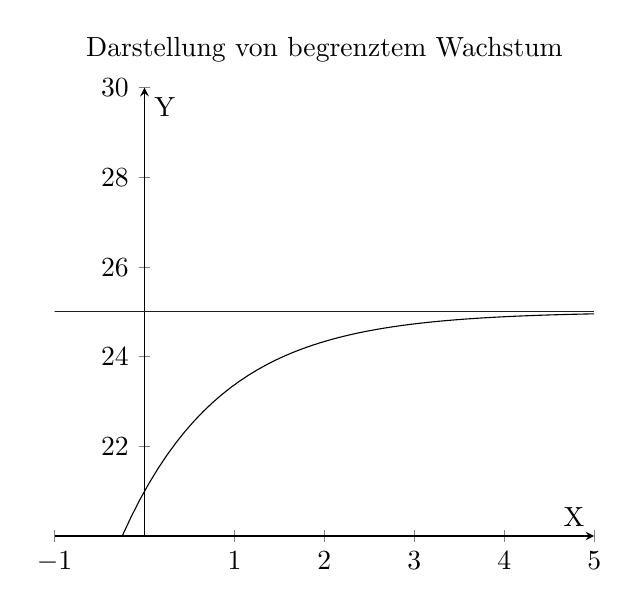
\begin{tikzpicture}
		\begin{axis}[
		title={Darstellung von begrenztem Wachstum},
		axis lines=middle,
		clip=true,
		xlabel={X},
		ylabel={Y},
		xmin=-1,
		xmax=5,
		ymin=20,
		ymax=30
		]
		\addplot[samples=100]{25-4*(exp(-0.9*x))} node[right,pos=1]{$25-4e^{-0.9x}$};
		\addplot[color=blue, samples=100]{25} node[right,pos=1]{$25$};
		\end{axis}
	\end{tikzpicture}
	\caption{Der Graph von $25-4e^{-0.9x}$ konvergiert zu $25$}
\end{figure}

Die 25 Grad stellen das Minimum der Temperatur, welche der Kaffe erreichen kann, dar. Somit kann nur Abb 3 zutreffen auf eine mit einem begrenzten Wachstum. Um nun den Prozess des Modellierens, der Funktion, welche die Temperatur des Kaffes darstellt, fortzuführen, ist es wichtig sich die Informationen, welche gegeben sind, anzuschauen. So kann beispielsweise aus der Information, dass der Kaffe jeden Moment um 9\% wärmer wird, gezogen werden, dass $e^{-0.09}$ die alleinig um die Abnahme, sondern auch um die Begrenzung. Mit logischem Überlegen kann man nun den Graphen im Koordinatensystem verschieben. Dies erfolgt durch das Ändern der Parameter der Normalform. Da die Sättigungsgrenze bekannt ist, können wir mit dem Parameter $e$ den Graphen nach oben schieben, sodass der Graph bereits gegen $25$ konvergiert. Wissen wir nun den Startwert bzw. die Temperatur bei der wir den Kaffee raus gestellt haben, können wir konkret den Bereich der Wertemenge eingrenzen. Nehmen wir an, dass der Kaffe $4\deg$ kalt war, kann man sich nun den Bereich, der für die Rechnung relevant ist, berechnen. Dies wird mit der Hilfe von Subtraktion des Startwertes Minus die Sättigungsgrenze gemacht. Dies ist wichtig, weil wir einen Startwert benötigen für unsere Funktion. Normalerweise kann man einfach $a$ verändern, allerdings bedingt $-25$ diesen Wert. Unser Startwert ist also $25-4$. Daraus folgt, dass die Funktion wie folgt aussehen muss. \[f(x)=-21e^{-0.09x}+25\]
\section{Logisitisches Wachstum}



